%%%%%%%%%%%%%%%%%%%%%%%%%%%%%%%%%%%%%%%%%%%%%%%%%%%%%%
% A Beamer template for HKUST                        %
% Based on THU beamer theme                          %
% Author: Yuxuan HU                                  %
% Date: Aug 2024                                     %
% LPPL Licensed.                                     %
%%%%%%%%%%%%%%%%%%%%%%%%%%%%%%%%%%%%%%%%%%%%%%%%%%%%%%

\documentclass[serif, aspectratio=169]{beamer}
%\documentclass[serif]{beamer}  % for 4:3 ratio
\usepackage[T1]{fontenc} 
\usepackage{fourier} % see "http://faq.ktug.org/wiki/uploads/MathFonts.pdf" for other options
\usepackage{hyperref}
\usepackage{latexsym,amsmath,xcolor,multicol,booktabs,calligra}
\usepackage{graphicx,pstricks,listings,stackengine}
\usepackage{lipsum}

\author{Group7}
\title{ISOM5160 Group Report}
\subtitle{Dataset: amazon\_food\_reviews.csv}
\institute{
    \scriptsize
	\begin{tabular}{llll}
		\toprule
		% Name & SID & Name & SID  \\
		% \midrule
		CAO, Xi & 21271664 & LI, Heyi & 21265689  \\
		LIAO, Jingyu & 21262106 & LIN, Chuwei & 21237955  \\
		YE, Chenwei & 21199517 & ZHANG, Ziyang & 21266920  \\
		\bottomrule
	\end{tabular}
	\normalsize
}
\date{\small \today}
\usepackage{HKUSTstyle}

% defs
\def\cmd#1{\texttt{\color{red}\footnotesize $\backslash$#1}}
\def\env#1{\texttt{\color{blue}\footnotesize #1}}
% set colors
\definecolor{hkustyellow}{RGB}{167, 131, 55}
\definecolor{hkustblue}{RGB}{0, 56, 116}
\definecolor{hkustred}{RGB}{209, 51, 59}


\lstset{
    basicstyle=\ttfamily\small,
    keywordstyle=\bfseries\color{deepblue},
    emphstyle=\ttfamily\color{deepred},    % Custom highlighting style
    stringstyle=\color{deepgreen},
    numbers=left,
    numberstyle=\small\color{halfgray},
    rulesepcolor=\color{red!20!green!20!blue!20},
    frame=shadowbox,
}

%- --- --- --- --- --- --- --- --- --- --- --- --- --- --- --- 
\begin{document}

\begin{frame}
    \titlepage
    \vspace*{-0.6cm}
    \begin{figure}[htpb]
        \begin{center}
            
\includegraphics[keepaspectratio, scale=0.02]{pic/UST.png}
        \end{center}
    \end{figure}
\end{frame}

\begin{frame}    
\tableofcontents[sectionstyle=show,
subsectionstyle=show/shaded/hide,
subsubsectionstyle=show/shaded/hide]
\end{frame}

% Background & objective --- --- --- --- --- --- --- --- --- --- --- --- 

\section{Background \& Objective}
\begin{frame}{Background \& Objective}
	\begin{block}{Project background}
		\begin{itemize}
			\item Amazon product reviews contain a large amount of redundant and noisy information.
			\item It`s hard for merchant to get valuable insights and learn how to improve their product
		\end{itemize}
	\end{block}
	\begin{block}{Objective}
		\begin{itemize}
			\item Organize Amazon reviews and extract key informations (include sentiment, timeline information and goods key features extract)  so merchants know how to improve their products
		\end{itemize}
	\end{block}
\end{frame}

\section{Data Cleaning}

\begin{frame}{Data Cleaning}
	\begin{block}{Dirty data}
		\begin{itemize}
			\item Missing values in key fields (e.g., Text, Score, ProductId)
			\item Duplicate reviews (from same user /multiple Good reviews same product)
			\item Noisy , inconsistent text ,stop words will redundant the later works
		\end{itemize}
	\end{block}
    
	\begin{block}{Steps}
		\begin{itemize}
			\item Duplicate and blank value processing: Make product reviews unique and valid
			\item Unify text format and remove stop words: to facilitate subsequent sentiment analysis and keyword extraction
		\end{itemize}
	\end{block}
\end{frame}

\begin{frame}{Sentiment Analysis}
    
	\begin{block}{Why sentiment analysis?}
		\begin{itemize}
			\item The sentiment of some reviews is different from the actual review scores
			\item Provides merchants with actionable insights for product improvement
		\end{itemize}
	\end{block}
    
	\begin{block}{Steps}
		\begin{itemize}
			\item Model: Pre-trained BERT
			\item Download the pre-trained BERT model, download the data set for local training, and then score the original data for sentiment tendency
		\end{itemize}
	\end{block}

\end{frame}

\begin{frame}{Sentiment Analyze Result}
	
	\vspace{-5pt}
	\begin{figure}
		\centering
			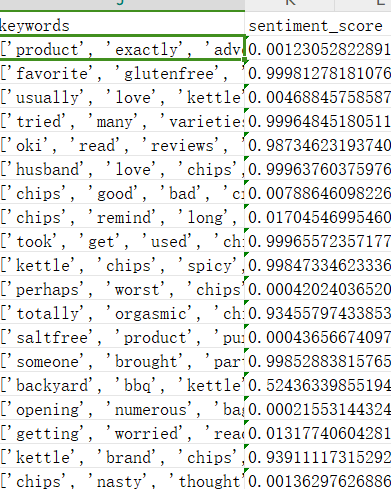
\includegraphics[height=6.5cm]{pic/dc.png}
		% \caption{Logo of the university.}
		% \label{fig:unilogo}
	\end{figure}

    \vspace{-5pt}
    \begin{center}
        \textbf{Added sentiment columns and keyword collections}
    \end{center}
    
\end{frame}

\section{Sentiment Analyze}

\begin{frame}{Sentiment Analyze}
    
	\begin{block}{Why sentiment analyze?}
		\begin{itemize}
			\item The sentiment of some reviews is different from the actual review scores
			\item Provides merchants with actionable insights for product improvement
		\end{itemize}
	\end{block}
    
	\begin{block}{Steps}
		\begin{itemize}
			\item Model: Pre-trained BERT
			\item Download the pre-trained BERT model, download the data set for local training, and then score the original data for sentiment tendency
		\end{itemize}
	\end{block}

\end{frame}

\begin{frame}{Sentiment-Rating Correlation \& Outlier Detection}
    
	\begin{block}{1. Methodology}
		\scriptsize
		\begin{itemize}
			\item Adjusted sentiment scores to match 5-point rating scale
			\item Computed Sentiment-Rating \textbf{Gap} = \textbf{Rating} - \textbf{Sentiment\_Score\_Scaled}
			\item Detected outliers with |Z| > 2 : 483/10819 ($ \approx ≈ 4.5\%$)
			\item \textbf{General Trend:} Ratings are \textbf{systematically higher} than sentiment scores. 
		\end{itemize}
	\end{block}
    
	\vspace{-20pt}
	\begin{figure}[htbp]
		\centering
		\begin{minipage}[t]{0.50\textwidth}
			\vspace{0pt}
			\centering
			\begin{figure}
				\centering
					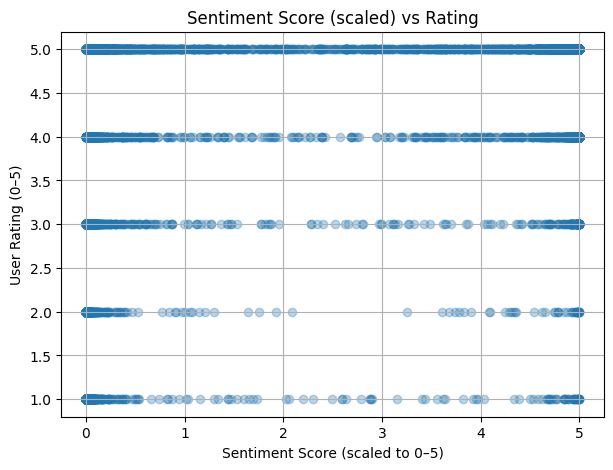
\includegraphics[height=4.5cm]{pic/sentiment_1.png}
			\end{figure}
		\end{minipage}
		\hfill
		\begin{minipage}[t]{0.49\textwidth}
			\vspace{0pt}
			\centering
			\begin{figure}
				\centering
					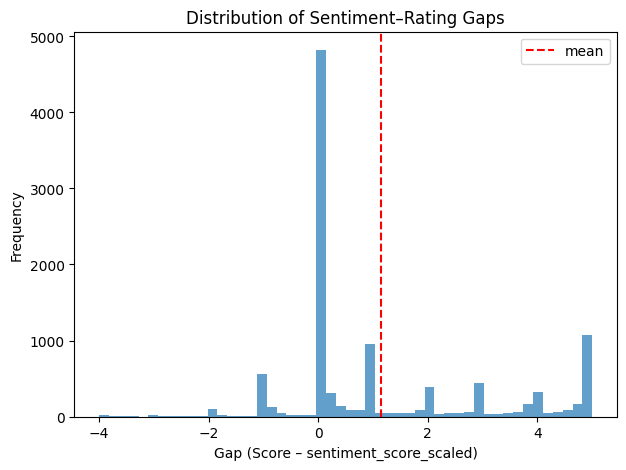
\includegraphics[height=4.5cm]{pic/sentiment_2.png}
			\end{figure}
		\end{minipage}
	\end{figure}

\end{frame}


\begin{frame}{Sentiment-Rating Correlation \& Outlier Detection}
    
	\scriptsize
	\begin{block}{2. Insights: Why Sentiment $\neq$ Rating}
		a. Text–Sentiment Model Bias
		\begin{itemize}
			\item Key words like "unfortunately", "so good", "used to be good" confuse sentiment detection.
			\item Context-dependent irony or comparison not captured by model.
		\end{itemize}

		\vspace{5pt}
		Example of the model bias:\\
		"the product was exactly \textbf{as advertised and fresh. unfortunately} i keep them in a candy dish in the office and they are going fast. we need to reorder to keep up with demand"
		
		\vspace{5pt}
		b. Human Behavior Factors
		\begin{itemize}
			\item Users express disappointment \textbf{politely}, often masking negative emotions.
			\item Positive service experience (e.g. refund) leads to positive feedback despite low product rating.
			\item Social courtesy bias: buyers avoid leaving harsh ratings or comments.
		\end{itemize}

		\vspace{5pt}
		Example of human behavior bias:\\
		"i was very angry about this but jr mushrooms has said they will \textbf{refund} me for the truffles and even let me keep them. so i \textbf{give jr credit for excellent responsiveness} and customer service, although i still feel they should not be labeled black winter truffles"
	\end{block}
    


\end{frame}











\section{Comment Time Series Analysis}


\begin{frame}{Comment Time Series Analysis}
	
	\vspace{-5pt}
	\begin{figure}
		\centering
			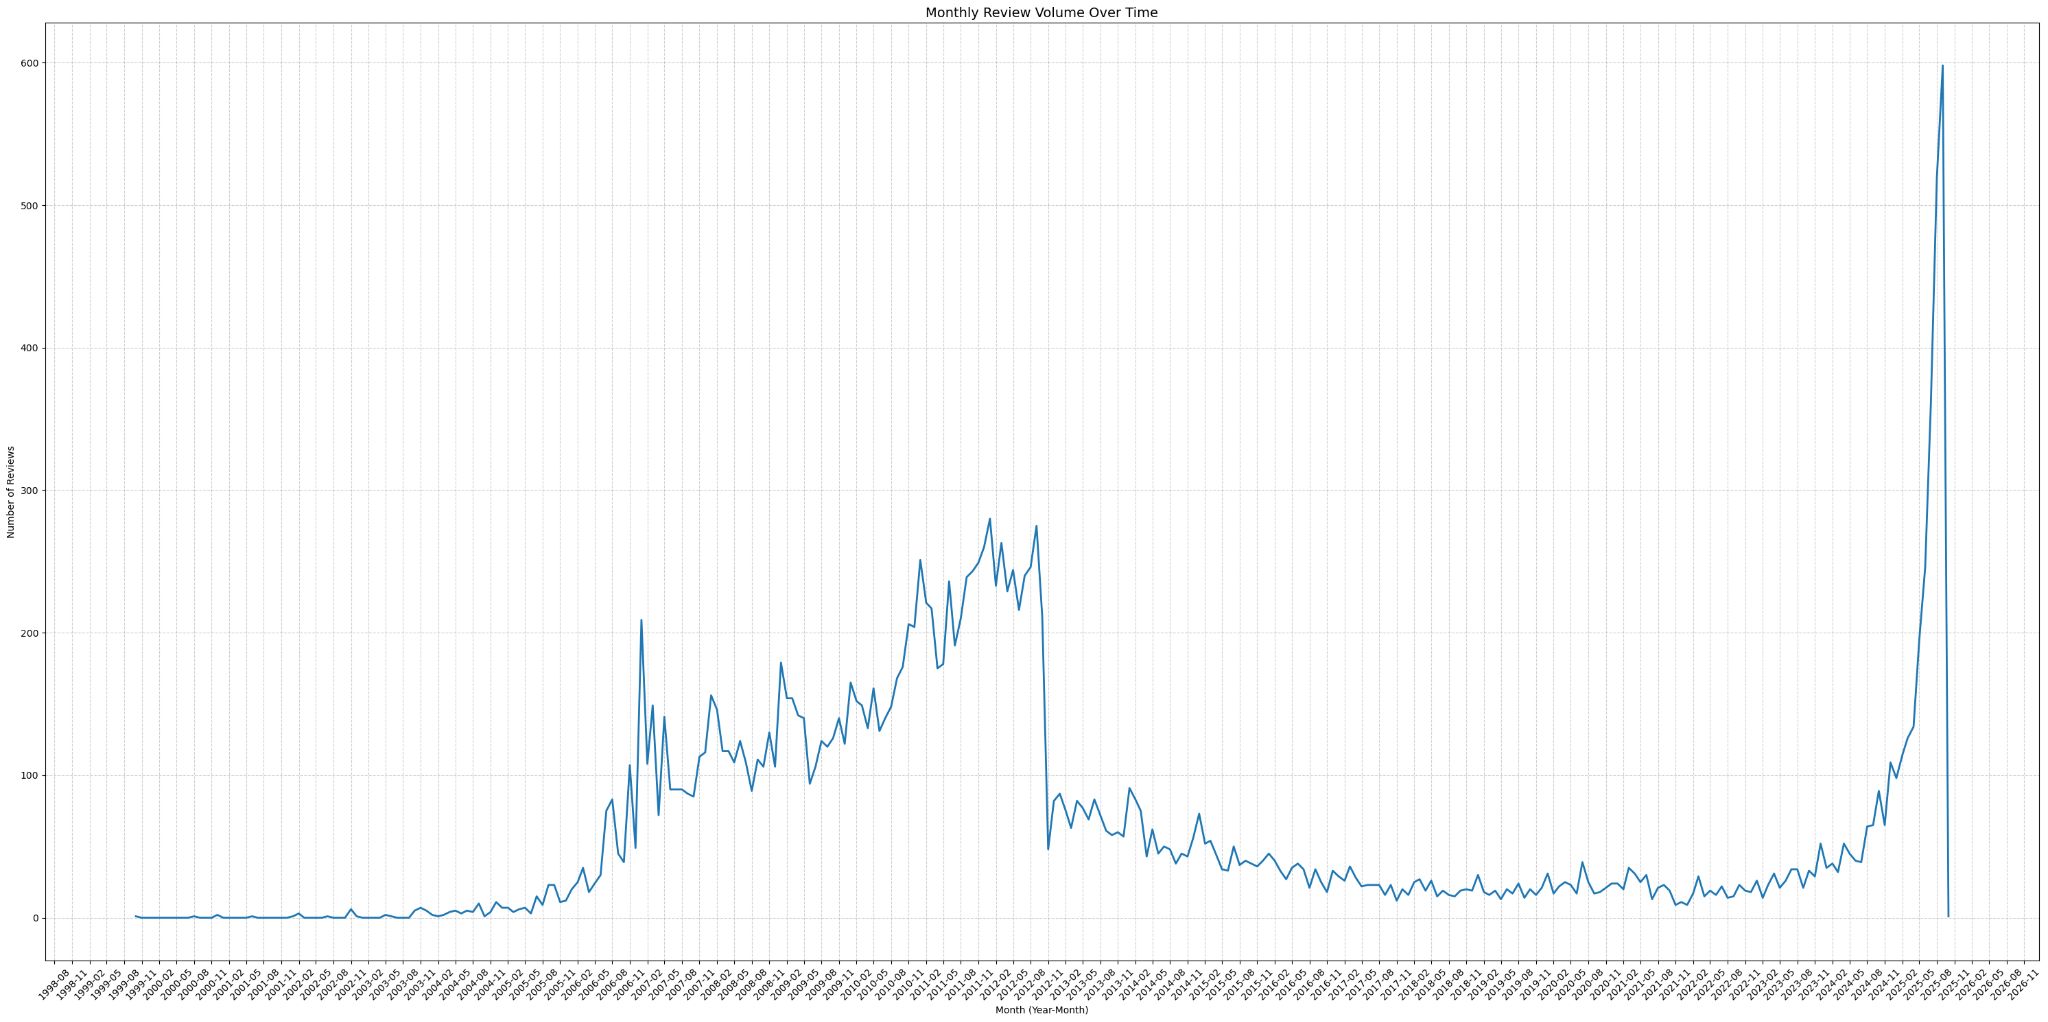
\includegraphics[height=6cm]{pic/ts_1.png}
		% \caption{Logo of the university.}
		% \label{fig:unilogo}
	\end{figure}

    \vspace{-5pt}
    \begin{center}
        \textbf{Review volume shows long-term growth, reflecting rising customer engagement.}
    \end{center}

\end{frame}

\begin{frame}{Comment Time Series Analysis}
	
	\vspace{-5pt}
	\begin{figure}
		\centering
			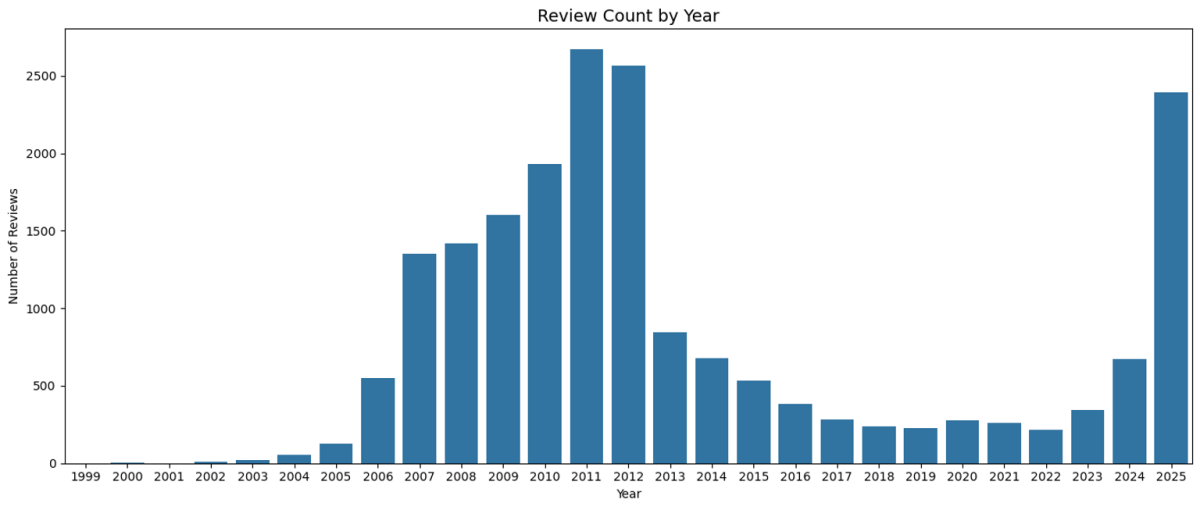
\includegraphics[height=6cm]{pic/ts_2.png}
		% \caption{Logo of the university.}
		% \label{fig:unilogo}
	\end{figure}

    \vspace{-5pt}
    \begin{center}
        \textbf{Yearly trends can help evaluate product lifecycle and marketing effectiveness.}
    \end{center}

\end{frame}

\begin{frame}{Comment Time Series Analysis}
	
	\vspace{-5pt}
	\begin{figure}
		\centering
			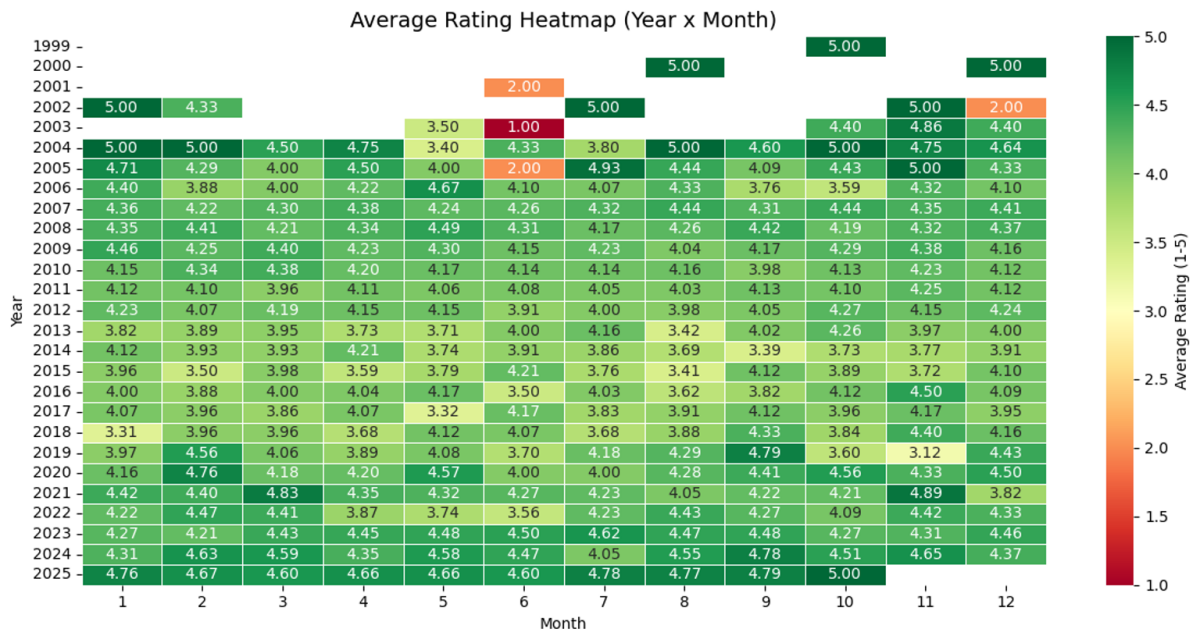
\includegraphics[height=6.5cm]{pic/ts_3.png}
		% \caption{Logo of the university.}
		% \label{fig:unilogo}
	\end{figure}

    \vspace{-5pt}
    \begin{center}
        \textbf{Ratings remain consistently positive, showing strong brand reputation.}
    \end{center}
    
\end{frame}

\section{Negative Review Analysis}

\begin{frame}{Negative Review Analysis}
    
	\begin{block}{Why need negative review analysis?}
		\begin{itemize}
			\item Assist in finding improvement directions(By knowing the distribution of negative reviews, decisions can be made to improve like supply chain, operations, preservation, transportation, and other aspects)
			\item Analyze the problems with the product(By knowing the distribution of negative reviews, decisions can be made to improve supply chain, operations, preservation, transportation, and other aspects)
		\end{itemize}
	\end{block}
    
	\begin{block}{Steps}
		\begin{itemize}
			\item Read the comment data after data cleaning
			\item Filter travel reviews through logical judgment
			\item Classify and analyze negative reviews based on keywords
		\end{itemize}
	\end{block}

\end{frame}

\begin{frame}{Negative Review Analysis}
    
	\begin{block}{Negative evaluation criteria}
		\scriptsize
		\begin{itemize}
			\item Accurately locate real negative reviews through dual filtering criteria
			\item Objective rating: Score <= 2 (considered low on a 5-point scale)
			\item Subjective sentiment: Sentimentscore < 0.4 (sentiment tendency score generated by data\_cleaning.py, below 0.4 is considered negative)
		\end{itemize}
	\end{block}
    
	\begin{block}{Keyword filtering}
		\scriptsize
		\begin{itemize}
			\item Map high-frequency keywords to 8 common negative cause categories in the food industry, and define the classification rules through the category\_mapping dictionary:
			\item Taste: such as taste, bitter, bland, etc
			\item Quality: such as poor, cheap, terrible, etc
			\item Expired (expired/spoiled): such as expired, rotten, mold, etc
			\item Other categories: packaging, price, delivery, quantity, smell
			\item Keywords that do not match the preset category are classified as' other ', ensuring that all keywords are categorized accordingly
		\end{itemize}
	\end{block}

\end{frame}




















\section{Correlation Between Ratings and Product Descriptions}

\begin{frame}{Correlation Between Ratings and Product Descriptions - Overview}
	% \frametitle<presentation>{Overview}

	\footnotesize

	\begin{block}{Steps}
		\begin{enumerate}
			\item Scrape supplementary data from amazon.com
			\item Analyse correlation for both visual \& text information
			\item \textbf{Correlation computation:} We use spearmanr to compute Correlation
		\end{enumerate}
	\end{block}
    
	\begin{block}{Part1. Visual Information Correlation}
		\begin{itemize}
			\item Correlation with the number of sample images
		\end{itemize}
	\end{block}
    
	\begin{block}{Part2. Text Information Correlation}
		\begin{itemize}
			\item Correlation with description length
			\item Correlation with reading ease
			\item Correlation with the marketing tone of the description
            \item Correlation with product description items
            % \emph{beamerarticle}
		\end{itemize}
	\end{block}
    
\end{frame}

\begin{frame}{Supplementary data (Scraped from Amazon's website)}
	
	\vspace{-5pt}
	\begin{figure}
		\centering
			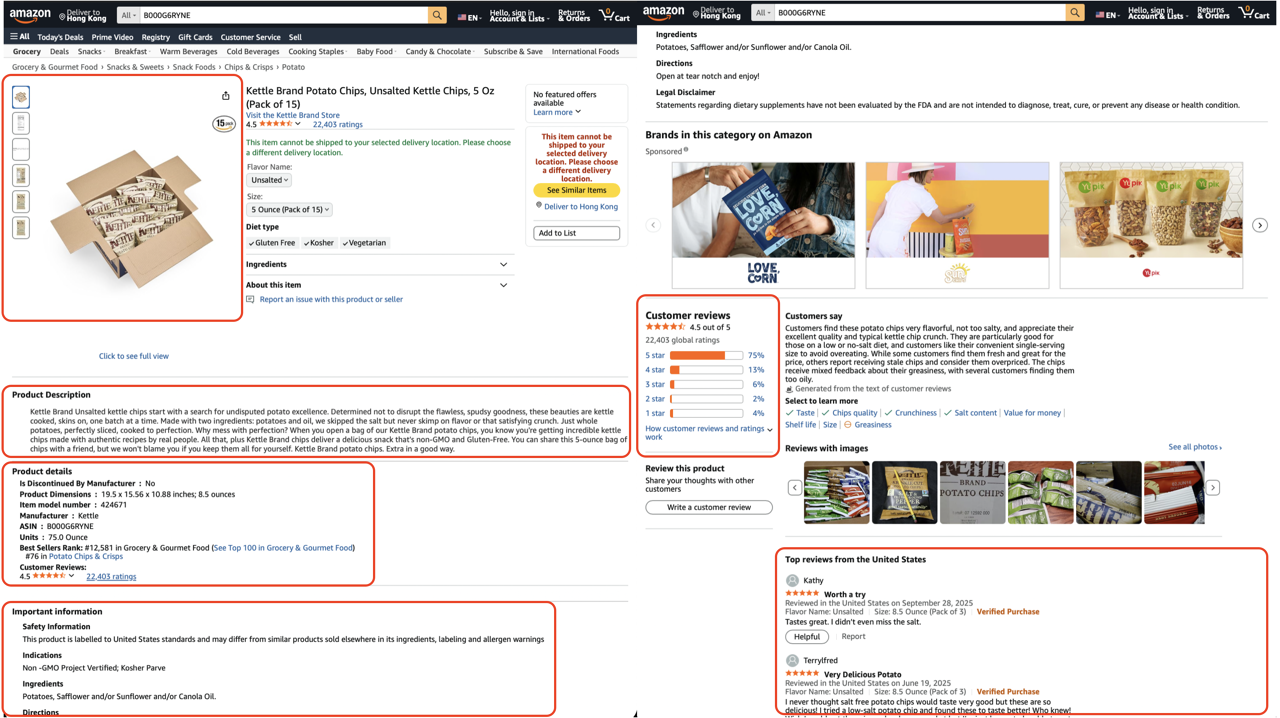
\includegraphics[height=7.3cm]{pic/collected_amazon_data.png}
		% \caption{Logo of the university.}
		% \label{fig:unilogo}
	\end{figure}

\end{frame}

\begin{frame}{Rating features}

	\begin{figure}
		\centering
			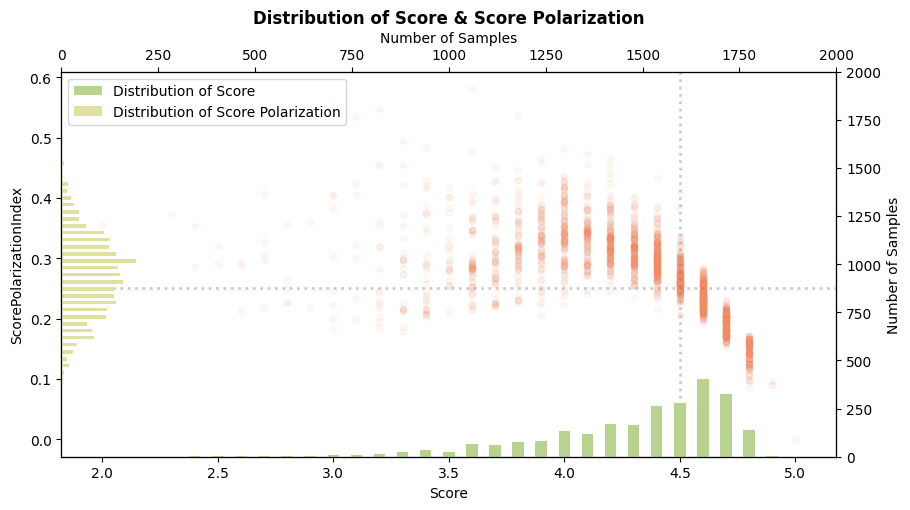
\includegraphics[height=5cm]{pic/score-scatter.png}
		% \caption{Logo of the university.}
		% \label{fig:unilogo}
	\end{figure}

    \begin{enumerate}
        \item \textbf{Mean Score:} The score displayed on the product detail page.
        \item \textbf{Score Polarization:} Indicates whether the ratings for this product are polarized.
        \item \textbf{Standards of Good Score:} Score >= 4.5; Polarization <= 0.25
    \end{enumerate}

\end{frame}
	
\begin{frame}{Correlation with the number of sample images}

	\begin{figure}
		\centering
			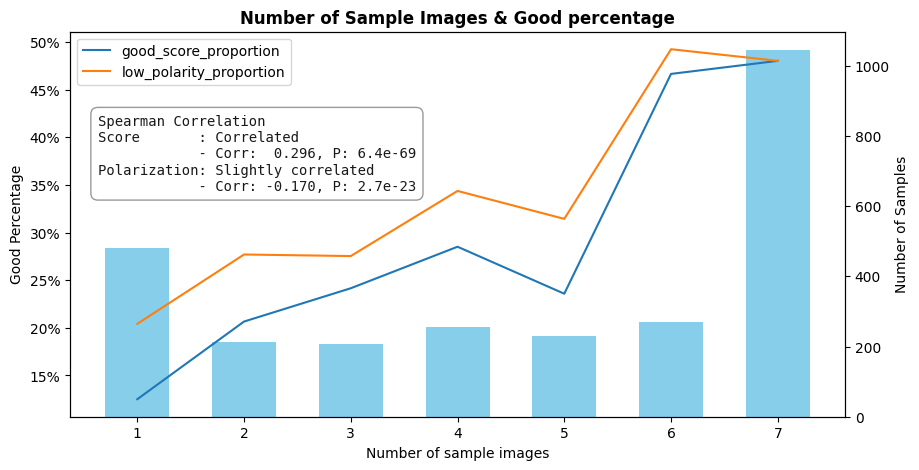
\includegraphics[height=5cm]{pic/corr_n_image.png}
		% \caption{Logo of the university.}
		% \label{fig:unilogo}
	\end{figure}

    \textbf{Conclusion:} The is a \underline{\textbf{positive correlation}} in product ratings and descriptions. The more images included in the description, the greater the likelihood of the product receiving positive reviews.

\end{frame}

\begin{frame}{Correlation with description length}

	\begin{figure}
		\centering
			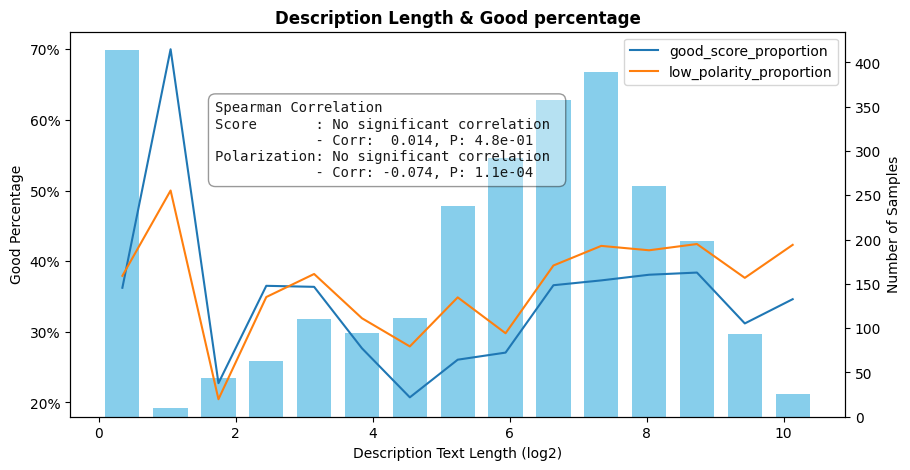
\includegraphics[height=5cm]{pic/corr_len_text.png}
		% \caption{Logo of the university.}
		% \label{fig:unilogo}
	\end{figure}

    \textbf{Conclusion:} There is \underline{\textbf{no significant correlation}} between product ratings and the length of product descriptions.

\end{frame}


\begin{frame}{Correlation with reading ease}

	\begin{figure}[htbp]
	\centering
	\begin{minipage}[t]{0.70\textwidth}
		\vspace{0pt}
		\centering
		\scriptsize
		\begin{tabular}{llrrl}
			\toprule
			ease\_index & compare\_with & corr & p\_value & conclusion \\
			\midrule
				flesch\_reading\_ease & Score & 0.0163 & 0.3863 & No significant correlation \\
				flesch\_reading\_ease & Polarization & -0.0187 & 0.3214 & No significant correlation \\
				flesch\_kincaid\_grade & Score & 0.0123 & 0.5135 & No significant correlation \\
				flesch\_kincaid\_grade & Polarization & -0.0130 & 0.4900 & No significant correlation \\
				gunning\_fog & Score & 0.0066 & 0.7270 & No significant correlation \\
				gunning\_fog & Polarization & -0.0076 & 0.6870 & No significant correlation \\
			\bottomrule
		\end{tabular}
		\normalsize
		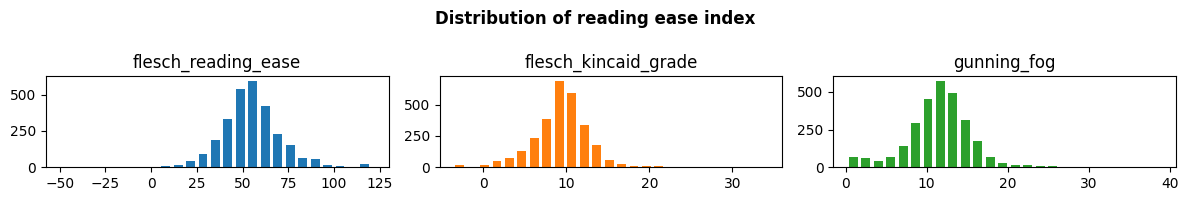
\includegraphics[height=1.86cm]{pic/corr_reading_ease_dist.png}
	\end{minipage}
	\hfill
	\begin{minipage}[t]{0.24\textwidth}
		\vspace{0pt}
		\centering
		\scriptsize
		\begin{itemize}
			\item \textbf{flesch reading ease:} The higher the score, the easier it is to read.
			\item \textbf{flesch kincaid grade:} The required grade level to read; The higher the number, the more difficult the reading level.
			\item \textbf{gunning fog:} Long word ratio; The higher the ratio, the harder it is to understand.
		\end{itemize}
		\normalsize
	\end{minipage}
	\end{figure}

	\textbf{Conclusion:} Product ratings show \underline{\textbf{no significant correlation}} with reading difficulty.

\end{frame}


\begin{frame}{Correlation with the marketing tone of the description}
	\vspace{-16pt}
	\begin{figure}[htbp]
		\centering
		\begin{minipage}[t]{0.50\textwidth}
			\vspace{0pt}
			\centering
			\tiny
			\begin{tabular}{llrrl}
				\toprule
				sentiment\_type & compare\_with & corr & p\_value & conclusion \\
				\midrule
				marketing\_tone\_score & Score & 0.0588 & 0.0007 & No significant correlation \\
				marketing\_tone\_score & Polarization & -0.0469 & 0.0066 & No significant correlation \\
				sentiment\_score & Score & 0.0788 & 0.0000 & No significant correlation \\
				sentiment\_score & Polarization & -0.0568 & 0.0010 & No significant correlation \\
				\bottomrule
			\end{tabular}
			\normalsize
		\end{minipage}
		\hfill
		\begin{minipage}[t]{0.36\textwidth}
			\vspace{0pt}
			\centering
			\begin{figure}
				\centering
					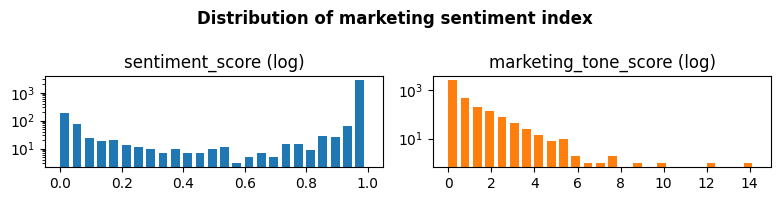
\includegraphics[height=1.45cm]{pic/corr_sentiment_dist.png}
			\end{figure}
		\end{minipage}
	\end{figure}

	\textbf{Types of marketing tone (Measuring Criteria):}
	\footnotesize
	\begin{enumerate}
		\item \textbf{marketing tone score:} The proportion of exaggerated marketing language in product descriptions. The higher the score, the more exaggerated the marketing claims become.
		\item \textbf{sentiment score by language model}: model is distilbert-base-uncased-finetuned-sst-2-english, The higher the score, the more positive the emotion.
	\end{enumerate}
	\normalsize

	\textbf{Conclusion:}
	\footnotesize
	\begin{itemize}
		\item Product ratings \underline{\textbf{show no significant correlation}} with marketing tone/sentiment.
		\item *However, since the metrics used to measure the emotional orientation of product descriptions do not follow a normal distribution, conclusions drawn from this basis may be unreliable.
	\end{itemize}
	\normalsize

\end{frame}


\begin{frame}{Correlation with product description items}
	\vspace{-16pt}
	\begin{figure}[htbp]
		\centering
		\begin{minipage}[t]{0.50\textwidth}
			\vspace{8pt}
			\centering
			\tiny
			\begin{tabular}{llrrl}
				\toprule
				item & compare\_with & corr & p\_value & conclusion \\
				\midrule
				Best Sellers Rank & Score & 0.3809 & 2.9e-116 & Highly correlated \\
				Directions & Score & 0.2211 & 2.12e-38 & Correlated \\
				Item model number & Score & 0.2721 & 4.95e-58 & Correlated \\
				Package Dimensions & Score & -0.2473 & 6.66e-48 & Correlated \\
				Package Dimensions & Polarization & 0.1717 & 1.32e-23 & Slightly correlated \\
				Product Dimensions & Score & 0.2715 & 9.67e-58 & Correlated \\
				Safety Information & Score & 0.1618 & 4.03e-21 & Slightly correlated \\
				\bottomrule
			\end{tabular}
			\normalsize
		\end{minipage}
		\hfill
		\begin{minipage}[t]{0.40\textwidth}
			\vspace{0pt}
			\centering
			\begin{figure}
				\centering
					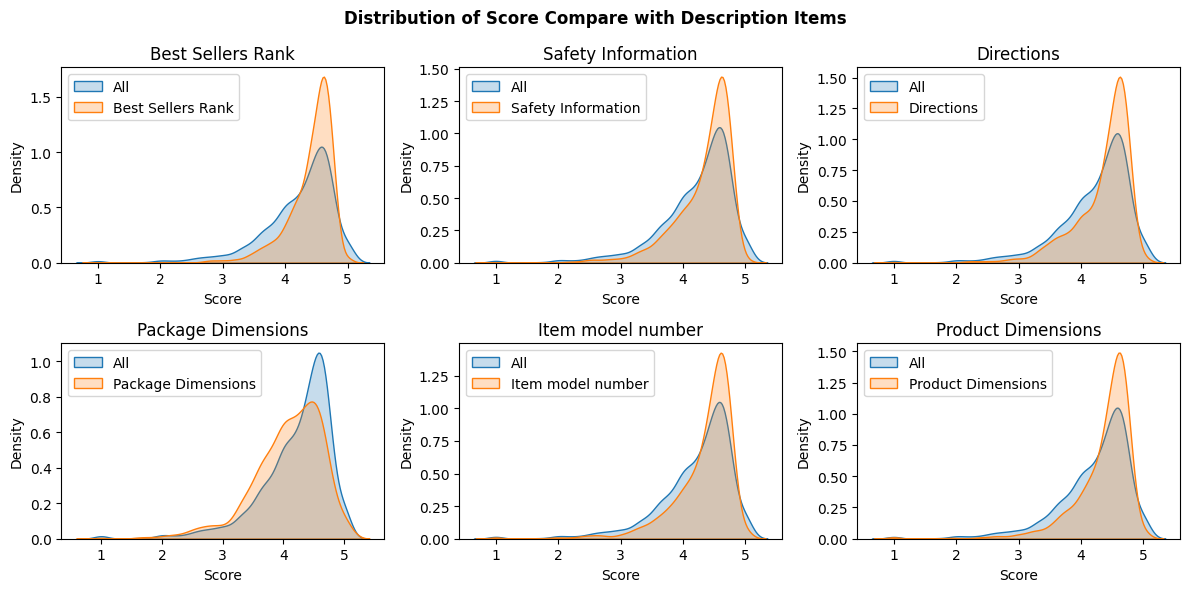
\includegraphics[height=3cm]{pic/corr_desc_item_dist.png}
			\end{figure}
		\end{minipage}
	\end{figure}

	\footnotesize
	\textbf{Products with the following description items might have a better rating:}
	\scriptsize
	\begin{itemize}
		\item \textbf{Best Sellers Rank:} Only high-quality goods carry this label.
		\item \textbf{Item model number \& Product Dimensions:} Products with model numbers may be more formal and reliable.
		\item \textbf{Directions:} Products accompanied by directions may reduce negative reviews caused by users' inability to use or misuse the product.
		\item \textbf{Safety Information:} Products with safety information may reduce negative reviews caused by user allergies.
	\end{itemize}
	\normalsize

	\footnotesize
	\textbf{Products with the following description items might have a lower rating:}
	\scriptsize
	\begin{itemize}
		\item \textbf{Package Dimensions:} May receive negative reviews due to logistics-related issues.
	\end{itemize}
	\normalsize

\end{frame}


% \begin{frame}{Chapter Conclusion}

% 	\begin{block}{For Sellers}
% 		\begin{itemize}
% 			\item Increase the number of product images;
% 			\item Make product descriptions as professional as possible;
% 			\item Provide more detailed safety information and instructions;
% 		\end{itemize}
% 	\end{block}

% 	\begin{block}{For Buyers}
% 		\begin{itemize}
% 			\item Choose products with more pictures;
% 			\item Choose products that appear more professional;
% 			\item Carefully read the product descriptions to avoid potential issues;
% 		\end{itemize}
% 	\end{block}

% \end{frame}





\section{Review Weighted Analysis}

\begin{frame}{Review Weighted Analysis}

	Remove outliers where HelpfulnessNumerator > HelpfulnessDenominator

	\vspace{-15pt}
	\begin{figure}[htbp]
		\centering
		\begin{minipage}[t]{0.50\textwidth}
			\vspace{0pt}
			\centering
			\[
			r = \frac{\text{HelpfulnessNumerator} + a}
					{\text{HelpfulnessDenominator} + a + b}
			\]
		\end{minipage}
		\hfill
		\begin{minipage}[t]{0.49\textwidth}
			\vspace{0pt}
			\centering
			\[
			t = 1 + \log(1 + \text{HelpfulnessDenominator})
			\]
		\end{minipage}
	\end{figure}

	\vspace{10pt}
	\textbf{Comment Weight:}

	\[
	\text{weighted\_mean} =
	\frac{\sum (\text{Score} \times \text{weight})}
		{\sum \text{weight}}
	\]

	
	\vspace{10pt}
    \textbf{Example:} If there are 10 five-star ratings with no votes and 1 one-star rating with 50 people finding it useful → the weighted mean will lean closer to one star.

\end{frame}



\begin{frame}{Review Weighted Analysis}

	\textbf{Bayesian Mean:}
	\[
	WeightedScore = \frac{v}{v + m} \cdot R + \frac{m}{v + m} \cdot C
	\]

	\vspace{10pt}

	\textbf{Optimized:}
	\[
	\frac{m \times \text{global\_mean} + \text{weighted\_mean} \times \sum \text{weight}}
		{m + \sum \text{weight}}
	\]

	\vspace{10pt}

    \textbf{Conclusion:} Based on the weighted mean, it converges toward the global average to avoid small-sample extremes. The fewer the reviews, the closer the Bayesian mean approaches the global average; Products with many reviews → the Bayesian mean approaches its own weighted mean.

\end{frame}



\begin{frame}{Review Weighted Analysis}

	\vspace{-15pt}
	\begin{figure}
		\centering
			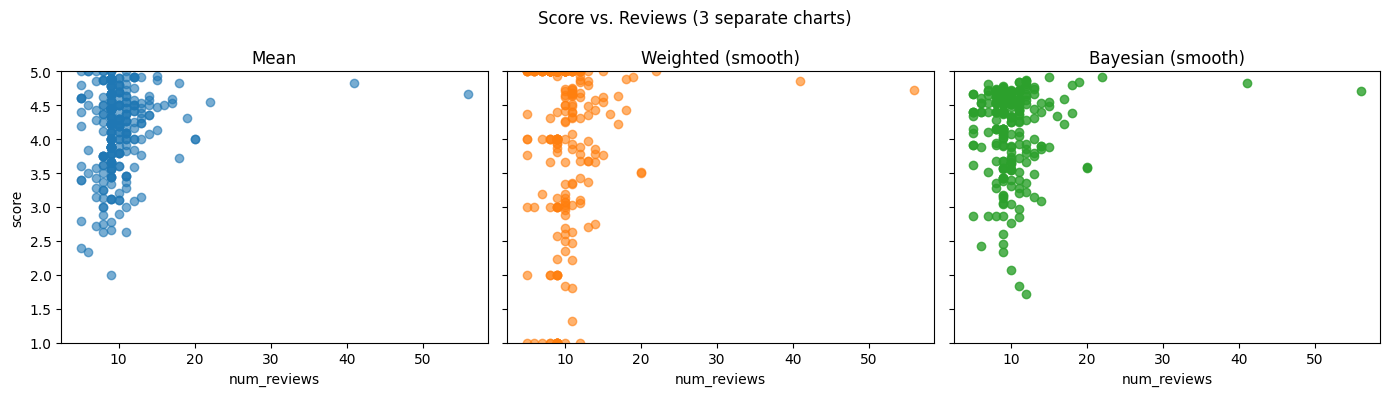
\includegraphics[height=4cm]{pic/weight_1.png}
	\end{figure}

    \textbf{Conclusion:} The raw mean is highly susceptible to bias when the sample size is small, easily skewed by a single extreme review. Weighted Smooth reduces the impact of noisy reviews. Bayesian Smooth applies “confidence contraction” to products with small sample sizes—bringing ratings closer to the global mean to prevent misrepresentation.

\end{frame}




% Results --- --- --- --- --- --- --- --- --- --- --- 
\section{Overall Takeaways}


\begin{frame}{Overall Takeaways}
    \footnotesize

    \begin{block}{Overall Takeaways for Merchants}
		\begin{itemize}
			\item \textbf{Listen Beyond the Stars} - Text sentiment often reveals issues hidden behind high scores.
            \item \textbf{Focus on Quality Signals} - Address taste, packaging, and logistics to curb negative reviews.
            \item \textbf{Professional Product Overview} - Include detailed, credible product information and visuals.
            \item \textbf{Leverage Weighted Analytics} - Use smoothed scores for fairer product comparisons.
            \item \textbf{Continuously Monitor Feedback Trends} - Use time-series tracking to align improvement with customer behavior.
		\end{itemize}
	\end{block}
    
	\begin{block}{Technical Contributions}
		\begin{itemize}
            \item \textbf{End-to-end review analysis pipeline} combining data cleaning, sentiment modeling, and statistical validation.
            \item \textbf{Hybrid NLP-statistical approach} ensuring both semantic accuracy and analytical robustness.
            \item \textbf{Practical insight generation} helping sellers understand reviews and improve their products.
		\end{itemize}
	\end{block}
\end{frame}

\begin{frame}
    \huge
    \begin{center}
        \textbf{Q \& A}
    \end{center}
\end{frame}


% --- Thank you slide ---
\begin{frame}

\begin{center}
{ 
    \huge
    Thank you for listening !
    \normalsize
}
\vspace{1cm}

Group 7 \\[3em]

\scriptsize
\begin{tabular}{llll}
    \toprule
    % Name & SID & Name & SID  \\
    % \midrule
    CAO, Xi & 21271664 & LI, Heyi & 21265689  \\
    LIAO, Jingyu & 21262106 & LIN, Chuwei & 21237955  \\
    YE, Chenwei & 21199517 & ZHANG, Ziyang & 21266920  \\
    \bottomrule
\end{tabular}
\normalsize
\end{center}
\end{frame}

\end{document}